\chapter{Results}
\label{ch:results}

\textbf{The results section needs to start with a summary of what the study is and what methods were used. someone should be able to read only your results and know exactly whats going on}

During the first run of my results I compared 15 different classification algorithm and scalier values taking the result with the best overall accuracy.
\begin{itemize}
\item include table of these results
\item The dataset I am using has 75 percent not cancelled bookings and 25 percent cancelled bookings
\end{itemize}



\begin{figure}[hbt!]
 %\centering
 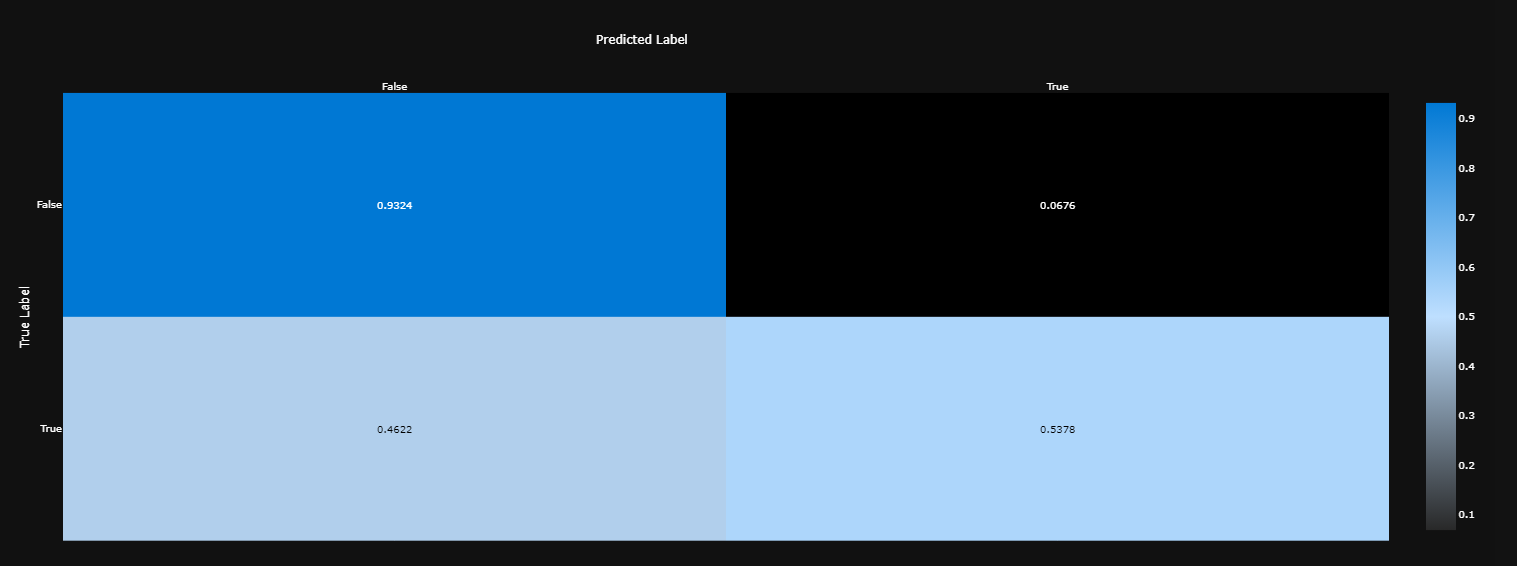
\includegraphics[width=10cm]{figures/azure_ml_confusion_matrix_xg.png}
 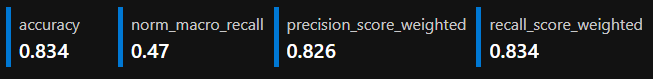
\includegraphics[width=10cm]{figures/xg_boost_scores.png}
 \caption{Confusion matrix from first run normalized}
\end{figure}


\begin{itemize}
\item A confusion matrix is a table that shows how well a classification model performs on a collection of test data for which the true values are known. The 4 sections that make up a confusion matrix are, true positives (TP) these are bookings that the model predicted as cancelled and are actually cancelled. True negatives (TN) these are bookings predicted correctly as not cancelled. False positives (FP) are bookings that the model predicted as cancelled but didn't and False negatives (FN) these are bookings the model predicted as not cancelled but did cancel. TP is the most important because this is where the model has predicted a booking as going  to cancel and has actually cancelled which is the objective of this research.
\item  The accuracy of a classification model is (TP+TN)/total. This is the number of bookings accurately classified as either cancelled or not cancelled, In this case it is more valuable to classify TP than TN since cancelled bookings are the focus of this research. figure \textbf{4.1} shows  0.93TF 0.54TP gives an overall accuracy of 0.83, this appears to be a very good result with over 80 percent of the bookings accurately predicted.
\item Recall is TP / (TP + FN), this is the proportion of actual positive values predicted correctly \textbf{figure 4.1} shows this is only 47 percent of true positive values are identified correctly. Showing that accuracy is not the most important metric here since with no true positive values predicted correctly the accuracy would still be 75 percent and the original problem statement has not been solved. 
\item knowing that Recall should be my primary metric to target and not accuracy using Azure ML I was able to change the target metric to Recall. \textbf{figure 4.3} shows the settings I applied with the new primary metric being norm macro recall. Setting the primary metric means Auto ML can optimise the model selection based on recall.
\item Include the results of the first run with azure ml - talk about all of the different algorithms and scalars used along with the number of cross validations
\item talk about K fold cross validation
\end{itemize}



During this run I used Azure ML to evaluate and compare multiple different algorithms

\begin{itemize}
\item knowing that I wanted to take the algorithm with the best recall I run Auto ML again keeping all other values the same, and only changing the primary metric 
\item same dataset and train test split
\item target metric changed to recall, meaning it evaluates and ranks the results differently 
\item what algorithms did it test this time
\item what is the accuracy, recall and precision
\end{itemize}

\begin{figure}[hbt!]
 %\centering
 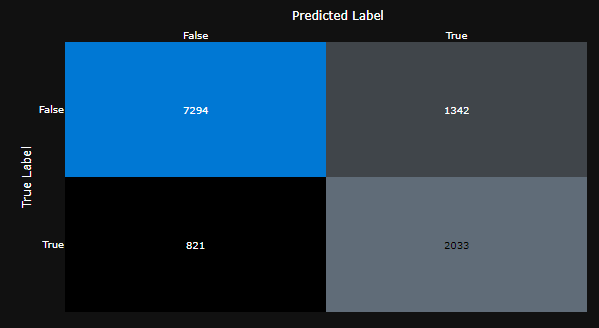
\includegraphics[width=10cm]{figures/azure_ml_confusion_matrix.png}
 \caption{Confusion matrix from final run of StackEnsemble algorithm, shows 71 percent recall}
\end{figure}

\begin{itemize}
\item do XGBoost vs StackedEnsemble, what is one better in this case
\item 
\end{itemize}


\begin{figure}[hbt!]
 %\centering
 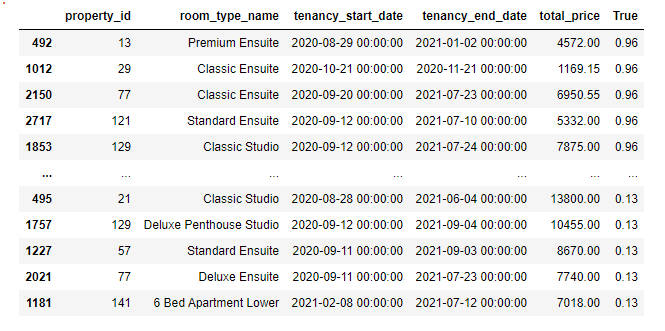
\includegraphics[width=10cm]{figures/canc_prob.png}
 \caption{prediction probability ranking each of the bookings made a chance of canceling}
\end{figure}

\begin{itemize}
\item classification is a value between 0 and 1, at over 0.5 booking gets classified as cancelled 
\item prediction probability is able to rank bookings made by there chance of cancelling 
\end{itemize}



